\chapter{Theory: The unsymmetric spectral element method}
\label{ch:theory}

This chapter describes the formulation as it is implemented in
\code{code/subroutines}. The literature is collected in \cref{ch:literature}.

\section{Problem}

The code solves linear plane elasticity on a domain $\Omega$ with thickness 1. In
Voigt notation, the equilibrium equation, Hooke's law and the strains read
\begin{equation}
  \matr L^{\T}\bm\sigma + \vect b = \vect 0,\qquad
  \bm\sigma = \matr C\,\bm\varepsilon,\qquad
  \bm\varepsilon = \matr L\,\vect u =
  \begin{bmatrix}\varepsilon_{xx}\\ \varepsilon_{yy}\\ \gamma_{xy}\end{bmatrix},
  \qquad
  \matr L = \begin{bmatrix}\partial_x & 0\\ 0 & \partial_y\\
                           \partial_y & \partial_x\end{bmatrix},
\end{equation}
where $\vect u$ is the displacement vector, $\bm\sigma$ and $\bm\varepsilon$ are
the stress and strain vectors, $\vect b$ is the body force per unit volume and
$\matr L$ is the differential operator, with prescribed displacements
$\bar{\vect u}$ on the Dirichlet boundary $\Gamma_\mathrm{u}$ and prescribed
tractions $\bar{\vect t}$ on the Neumann boundary $\Gamma_\mathrm{t}$. $\matr C$ is
the $3\times3$ plane stress matrix (\code{HookeMatrix2d}, or condensed from the
three-dimensional Hooke matrix with \code{PlaneStressConstitutiveMatrices}).

\section{Petrov-Galerkin weak form}

The classical (Bubnov-Galerkin) finite or spectral element uses the same
isoparametric shape functions to interpolate the displacements (trial
functions) and to weight the equilibrium equation (test functions). The
unsymmetric element uses two different sets \parencite{Rajendran2010technique},
see \cref{tab:spaces,fig:spaces}.

\begin{table}[htbp]
  \centering
  \caption{Shape functions of the unsymmetric element.}
  \label{tab:spaces}
  \begin{tabular}{@{}lll@{}}
    \toprule
    Role & Shape functions & Property \\
    \midrule
    test (weighting) & parametric, $N_i(\xi,\eta)$ &
      continuous across element edges \\
    trial (displacement) & metric, $M_j(x,y)$ &
      complete polynomials in $x$ and $y$ \\
    \bottomrule
  \end{tabular}
\end{table}

\begin{figure}[htbp]
  \centering
  % Reference element (parametric test functions) and distorted element with
% corotational skew coordinates (metric trial functions)
\begin{tikzpicture}[every node/.style={font=\small}]
  % ---- reference element ----
  \begin{scope}[scale=1.1]
    \draw[thick, fill=black!4] (-1,-1) rectangle (1,1);
    \draw[dimarrow] (0,0) -- (1.5,0) node[right] {$\xi$};
    \draw[dimarrow] (0,0) -- (0,1.5) node[above] {$\eta$};
    \node[node dot] at (0,0) {};
    \node at (0,-1.45) {reference element $\hat\Omega=[-1,1]^2$};
    \node[align=center] at (0,-2.05) {test functions $N_i(\xi,\eta)$\\(parametric, conforming)};
  \end{scope}
  % ---- mapping ----
  \draw[-{Stealth[length=3mm]}, thick] (2.0,0.4) to[bend left=25]
    node[above] {$\vect x(\xi,\eta)=\sum_k N_k(\xi,\eta)\,\vect x_k$} (5.0,0.4);
  % ---- distorted element ----
  \begin{scope}[shift={(5.4,-1.6)}]
    \coordinate (A) at (0,0);
    \coordinate (B) at (3.4,0.5);
    \coordinate (C) at (3.0,3.0);
    \coordinate (D) at (0.4,2.4);
    \draw[thick, fill=black!4] (A) .. controls (1.7,-0.5) .. (B) -- (C)
      .. controls (1.6,3.3) .. (D) -- cycle;
    % element centre x0 = x(0,0) and skew axes along dx/dxi, dx/deta
    \coordinate (X0) at (1.72,1.53);
    \node[node dot, label={[label distance=-2pt]below left:$\vect x_0$}] at (X0) {};
    \draw[dimarrow, very thick, blue!60!black] (X0) -- ++(1.45,0.05) node[right] {$s$};
    \draw[dimarrow, very thick, blue!60!black] (X0) -- ++(0.2,1.2) node[above] {$t$};
    % global frame
    \draw[dimarrow] (-0.6,-0.6) -- (0.2,-0.6) node[right] {$x$};
    \draw[dimarrow] (-0.6,-0.6) -- (-0.6,0.2) node[above] {$y$};
    \node[align=center] at (1.7,-1.25) {trial functions $M_j(s,t)$\\(metric, complete in $x,y$)};
    \node[align=left, font=\footnotesize] at (5.15,1.5)
      {$\begin{bmatrix}s\\t\end{bmatrix}=\matr J_0^{-\T}(\vect x-\vect x_0)$\\[2pt]
       $\matr J_0=\left.\dfrac{\partial(x,y)}{\partial(\xi,\eta)}\right|_{(0,0)}$};
  \end{scope}
\end{tikzpicture}

  \caption{Parametric test functions are defined on the reference element,
    metric trial functions in the corotational skew coordinates $(s,t)$ of the
    physical element.}
  \label{fig:spaces}
\end{figure}

The displacements are interpolated with the metric functions, the virtual
displacements with the parametric functions. The principle of virtual work then
reads
\begin{equation}
  \int\limits_{\Omega} \bm\varepsilon(\vect w)^{\T}\matr C\,\bm\varepsilon(\vect u)\dd\Omega
  = \int\limits_{\Omega} \vect w^{\T}\vect b\dd\Omega
  + \int\limits_{\Gamma_\mathrm{t}} \vect w^{\T}\bar{\vect t}\dd\Gamma
  \label{eq:weakform}
\end{equation}
for every virtual displacement $\vect w$ (parametric) that vanishes on
$\Gamma_\mathrm{u}$. Both sets of shape functions are interpolatory at the same
nodes, so the nodal displacements are the unknowns, as in the classical element.
Because the two sides of the weak form use different functions, the element
matrices are \emph{unsymmetric}.

\subsection*{Why the element is insensitive to mesh distortion}

If the exact displacement field is a polynomial of total degree $\le p$ in
$(x,y)$, where $p$ is the polynomial degree of the element, the metric functions
reproduce it exactly on every element, whatever its shape, so the strains and
stresses are exact as well. The parametric test functions are continuous across
the element edges, so the exact stresses satisfy the weak form \eqref{eq:weakform}
with these test functions (this is the principle of virtual work for the exact
solution). Hence the exact nodal values solve the discrete equations: the solution
is exact on any mesh, provided the integrals are evaluated exactly
(\cref{sec:quadrature}). This is the distortion immunity of Rajendran's
unsymmetric elements \parencite{Rajendran2003novel,Rajendran2010technique}, here
for arbitrary $p$. The classical isoparametric element loses this property as soon
as the element geometry is not a parallelogram, because the isoparametric
functions then no longer contain all polynomials of degree $p$ in $(x,y)$;
quadratic fields on elements with curved edges are the standard example
\parencite{Lee1993effects}. The metric functions need not be continuous across
element edges; continuity is provided by the test functions.

\section{Parametric (test) shape functions}

\code{ShapeFunctions2D_SEM(xi, eta, p)} builds products of one-dimensional
Lagrange polynomials through $p+1$ Gauss-Lobatto-Legendre (GLL) nodes in each
direction (\code{nodal_distribution.m}).

\paragraph{Geometry.} The element geometry is described with the same degree-$p$
shape functions as the displacements. The positions of the element
nodes, however, are computed from the 4-node (bilinear) or 8-node (Serendipity)
element of the input mesh (\code{pSpectralElement_NodesTopology}): every node is
placed at the image of its reference coordinates under the bilinear or
Serendipity map of the input element. The geometry is therefore the bilinear or
Serendipity geometry of the input mesh, whatever $p$ is: edges are straight
(4-node input) or parabolic (8-node input, $p\ge2$). The elements are subparametric
for $p>2$. For the thick cylinder, \code{studies/thick_cylinder/matlab/cyl_model.m}
places the nodes of the arcs on the exact geometry by Gordon-Hall blending.

\paragraph{Local node numbering.}
For degree $p$ an element has $(p+1)^2$ nodes: the 4 corners, then the interior
nodes of edge~1 ($\eta=-1$), edge~2 ($\xi=+1$), edge~3 ($\eta=+1$) and edge~4
($\xi=-1$), each in the direction of increasing $\xi$ or $\eta$, and finally the
interior nodes row by row ($\xi$ fastest), see \cref{fig:nodes}. Global degrees
of freedom (DOFs) are interleaved: node $n$ has $u_x$ at DOF $2n-1$ and $u_y$ at DOF
$2n$ (\code{Topology_DoF_2D}).

\begin{figure}[htbp]
  \centering
  % Local node numbering of a spectral element, p = 3, GLL nodes
\begin{tikzpicture}[scale=2.2, every node/.style={font=\small},
                    num/.style={inner sep=1.5pt}]
  \def\g{0.4472136}
  % element and node lines
  \draw[thick] (-1,-1) rectangle (1,1);
  \foreach \c in {-\g,\g} {
    \draw[densely dotted, black!40] (\c,-1) -- (\c,1);
    \draw[densely dotted, black!40] (-1,\c) -- (1,\c);
  }
  % nodes: (xi, eta, number, label position); labels of boundary nodes
  % point outwards, labels of interior nodes to the upper right
  \foreach \x/\y/\n/\pos in {
      -1/-1/1/below left, 1/-1/2/below right, 1/1/3/above right, -1/1/4/above left,
      -\g/-1/5/below, \g/-1/6/below,
      1/-\g/7/right, 1/\g/8/right,
      -\g/1/9/above, \g/1/10/above,
      -1/-\g/11/left, -1/\g/12/left,
      -\g/-\g/13/above right, \g/-\g/14/above right,
      -\g/\g/15/above right, \g/\g/16/above right} {
    \node[node dot] at (\x,\y) {};
    \node[num, \pos=2.5pt] at (\x,\y) {\n};
  }
  % edge labels (outside the node numbers)
  \node at (0,-1.32) {edge 1 ($\eta=-1$)};
  \node[rotate=90] at (1.36,0) {edge 2 ($\xi=+1$)};
  \node at (0,1.32) {edge 3 ($\eta=+1$)};
  \node[rotate=90] at (-1.36,0) {edge 4 ($\xi=-1$)};
  % local coordinate axes
  \draw[dimarrow] (-1.75,-1.55) -- (-1.3,-1.55) node[right] {$\xi$};
  \draw[dimarrow] (-1.75,-1.55) -- (-1.75,-1.1) node[above] {$\eta$};
\end{tikzpicture}

  \caption{Local node numbering of a spectral element of degree $p=3$ (GLL nodes).}
  \label{fig:nodes}
\end{figure}

\section{Metric (trial) shape functions in skew coordinates}

\code{ShapeFunctions2D_Metric(xQ, yQ, xN, yN, p)} builds shape functions that
are interpolatory at the element nodes $(x_k,y_k)$ in physical space, in four
steps:
\begin{enumerate}
  \item \textbf{Skew coordinates} (\code{CorotationalSkewCoordinates},
    \cite{Xie2016Modified}; \cite{Yuan1993New}). The skew coordinates $(s,t)$
    are Cartesian coordinates measured along the two element axes at the element
    centre, scaled with the element size: with the centre
    $\vect x_0 = \vect x(0,0)$ and the Jacobian $\matr J_0$ there,
    \begin{equation}
      \begin{bmatrix} s\\ t\end{bmatrix} = \matr J_0^{-\T}\,(\vect x - \vect x_0).
    \end{equation}
    They are linear in $x$ and $y$, move and rotate with the element, and
    coincide with $(\xi,\eta)$ on a parallelogram.
  \item \textbf{Polynomial space.} The shape functions are polynomials of degree
    $p_\upxi$ in $s$ and $p_\upeta$ in $t$ (all products $s^a t^b$ with $a\le
    p_\upxi$, $b\le p_\upeta$, the space $\mathcal Q_p(s,t)$). For good conditioning they
    are written in a Lagrange basis $\ell_a(\tilde s)\,\ell_b(\tilde t)$, where
    $\tilde s$, $\tilde t$ are the skew coordinates scaled to the interval
    $[-1,1]$ of the nodes; the shape functions themselves do not depend on the
    basis (\cref{ch:metric-basis}).
  \item \textbf{Interpolation.} The coefficients follow from the conditions
    $M_j(\vect x_k) = \delta_{jk}$ at the nodes, a linear system with the
    generalized Vandermonde matrix $\matr V$ (values of the basis at the nodes).
  \item \textbf{Derivatives.} The derivatives with respect to $x$ and $y$
    follow from those with respect to $s$ and $t$ with the constant matrix
    $\matr J_0^{-1}$.
\end{enumerate}
Properties (all covered by \code{tests/unit/MetricShapeFunctionsTest.m}):
\begin{itemize}
  \item \textbf{Completeness.} $s$ and $t$ are linear in $x$ and $y$, so every
    polynomial of total degree $\le p$ in $(x,y)$ is a polynomial of degree $\le p$
    in $(s,t)$ and is reproduced exactly on any element shape.
  \item \textbf{Frame invariance.} Rigid-body motions and uniform scaling of the
    element do not change the shape functions.
  \item \textbf{Affine elements.} On a parallelogram the metric and the
    parametric functions coincide, so the element is the classical spectral
    element and $\matr K_e$ is symmetric.
  \item \textbf{Unisolvence.} The interpolation conditions can be singular for
    special node positions on strongly distorted elements, e.g.\ when two nodes
    coincide \parencite{Ooi2008Remedies}. The code stops with an error in this
    case (\code{CheckUnisolvent}), and the studies report such elements as
    rejected.
\end{itemize}

\code{method=2} (\code{p.metricMethod=2}) uses the hybrid space instead of
$\mathcal Q_p(s,t)$: all polynomials of total degree $\le m=\min(p_\upxi,p_\upeta)$ in
the scaled skew coordinates $(\tilde s,\tilde t)$, $\mathcal P_m(\tilde s,\tilde t)$,
complemented by parametric functions of $(\xi,\eta)$
(\cref{sec:metric-hybrid}). It has the same
completeness and invariance, equals the parametric space on all straight-edged
elements and avoids the exponential growth of the Lebesgue constant of
$\mathcal Q_p(s,t)$ on distorted elements.

\section{Element stiffness matrix}

The Jacobian is used in the convention (\code{Jacobi_Matrix})
\begin{equation}
  \matr J = \begin{bmatrix} \partial x/\partial\xi & \partial y/\partial\xi\\
                            \partial x/\partial\eta & \partial y/\partial\eta
            \end{bmatrix}.
\end{equation}
The stiffness matrix (\code{Ke_2D}, vectorized in
\code{studies/thick_cylinder/matlab/cyl_Ke_PM.m}) reads
\begin{equation}
  \matr K_e = \int\limits^{1}_{-1}\int\limits^{1}_{-1}\matr B_\mathrm{L}^{\T}\matr C\,
  \matr B_\mathrm{R}\,\det(\matr J)\dd\xi\dd\eta,
\end{equation}
where $\matr B_\mathrm{L}$ holds the derivatives of the parametric (test) and
$\matr B_\mathrm{R}$ those of the metric (trial) functions. The product
$\det(\matr J)\,\matr B_\mathrm{L}$ is computed with the adjugate of $\matr J$,
$\det(\matr J)\,\matr J^{-1}$, so $\det(\matr J)$ never appears in a
denominator; this is Rajendran's third condition for distortion immunity.
$\matr B_\mathrm{R}$ is evaluated at the physical positions of the Gauss points.
Consequences:
\begin{itemize}
  \item Rigid-body modes lie in both the right and the left null space of
    $\matr K_e$, and $\operatorname{rank}(\matr K_e) = n_\mathrm{dof}-3$, where
    $n_\mathrm{dof}$ is the number of DOFs of the element.
  \item $\matr K_e$ is unsymmetric unless the element is a parallelogram.
\end{itemize}

\subsection*{Numerical integration}
\label{sec:quadrature}

\code{Ke_2D} uses $2p_\upxi\times2p_\upeta$ Gauss-Legendre points by default (other
numbers can be passed); the mesh-level studies of the paper use calibrated rules
(\code{manuscript/studies/ms_rule.m}). Whether a rule integrates the element matrix
exactly depends on the element shape, because the metric functions are polynomials
in $(x,y)$, and $x$, $y$ and $\det(\matr J)$ are polynomials in $(\xi,\eta)$ whose
degree grows with the distortion. The integrands of the trial space
$\mathcal Q_p(s,t)$ are polynomials in $(\xi,\eta)$, so a finite Gauss rule is exact;
its size was determined numerically (smallest rule that reproduces the matrix of a
40-point rule to $10^{-12}$, single elements of \cref{fig:test-elements}):
\begin{center}
  \begin{tabular}{@{}lcc@{}}
    \toprule
    element (input mesh) & $\matr K_e$ exact with & $2p$ sufficient? \\
    \midrule
    parallelogram & $p+1$ & yes \\
    straight edges (4-node) & $\lceil 3p/2\rceil$ & yes \\
    curved edges (8-node), $p\ge2$ & $2p+1$ to $2p+2$ & no \\
    \bottomrule
  \end{tabular}
\end{center}
\begin{figure}[htbp]
  \centering
  % Single test elements (tests/helpers/usemTestElement.m); generated
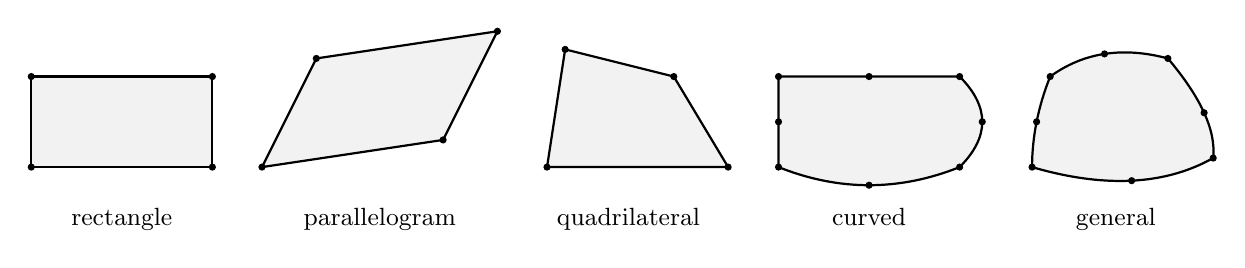
\begin{tikzpicture}[x=1.15cm, y=1.15cm, every node/.style={font=\small}]
  \begin{scope}[xshift=0.00cm]
    \draw[thick, fill=black!5] (0.0000,0.0000) -- (2.0000,0.0000) -- (2.0000,1.0000) -- (0.0000,1.0000) -- cycle;
    \fill (0.0000,0.0000) circle (1.3pt);
    \fill (2.0000,0.0000) circle (1.3pt);
    \fill (2.0000,1.0000) circle (1.3pt);
    \fill (0.0000,1.0000) circle (1.3pt);
    \node[below] at (1.000,-0.35) {rectangle};
  \end{scope}
  \begin{scope}[xshift=2.93cm]
    \draw[thick, fill=black!5] (0.0000,0.0000) -- (2.0000,0.3000) -- (2.6000,1.5000) -- (0.6000,1.2000) -- cycle;
    \fill (0.0000,0.0000) circle (1.3pt);
    \fill (2.0000,0.3000) circle (1.3pt);
    \fill (2.6000,1.5000) circle (1.3pt);
    \fill (0.6000,1.2000) circle (1.3pt);
    \node[below] at (1.300,-0.35) {parallelogram};
  \end{scope}
  \begin{scope}[xshift=6.55cm]
    \draw[thick, fill=black!5] (0.0000,0.0000) -- (2.0000,0.0000) -- (1.4000,1.0000) -- (0.2000,1.3000) -- cycle;
    \fill (0.0000,0.0000) circle (1.3pt);
    \fill (2.0000,0.0000) circle (1.3pt);
    \fill (1.4000,1.0000) circle (1.3pt);
    \fill (0.2000,1.3000) circle (1.3pt);
    \node[below] at (0.900,-0.35) {quadrilateral};
  \end{scope}
  \begin{scope}[xshift=9.49cm]
    \draw[thick, fill=black!5] (0.0000,0.0000) .. controls (0.6667,-0.2667) and (1.3333,-0.2667) .. (2.0000,0.0000) .. controls (2.3333,0.3333) and (2.3333,0.6667) .. (2.0000,1.0000) .. controls (1.3333,1.0000) and (0.6667,1.0000) .. (0.0000,1.0000) .. controls (0.0000,0.6667) and (0.0000,0.3333) .. (0.0000,0.0000) -- cycle;
    \fill (0.0000,0.0000) circle (1.3pt);
    \fill (2.0000,0.0000) circle (1.3pt);
    \fill (2.0000,1.0000) circle (1.3pt);
    \fill (0.0000,1.0000) circle (1.3pt);
    \fill (1.0000,-0.2000) circle (1.3pt);
    \fill (2.2500,0.5000) circle (1.3pt);
    \fill (1.0000,1.0000) circle (1.3pt);
    \fill (0.0000,0.5000) circle (1.3pt);
    \node[below] at (1.000,-0.35) {curved};
  \end{scope}
  \begin{scope}[xshift=12.71cm]
    \draw[thick, fill=black!5] (0.0000,0.0000) .. controls (0.8000,-0.2333) and (1.4667,-0.2000) .. (2.0000,0.1000) .. controls (2.0333,0.4000) and (1.8667,0.7667) .. (1.5000,1.2000) .. controls (1.0000,1.3333) and (0.5667,1.2667) .. (0.2000,1.0000) .. controls (0.0667,0.6667) and (0.0000,0.3333) .. (0.0000,0.0000) -- cycle;
    \fill (0.0000,0.0000) circle (1.3pt);
    \fill (2.0000,0.1000) circle (1.3pt);
    \fill (1.5000,1.2000) circle (1.3pt);
    \fill (0.2000,1.0000) circle (1.3pt);
    \fill (1.1000,-0.1500) circle (1.3pt);
    \fill (1.9000,0.6000) circle (1.3pt);
    \fill (0.8000,1.2500) circle (1.3pt);
    \fill (0.0500,0.5000) circle (1.3pt);
    \node[below] at (0.925,-0.35) {general};
  \end{scope}
\end{tikzpicture}

  \caption{Single test elements of the element tests, of the element studies of the
    paper and of the table on numerical integration
    (\texttt{usemTestElement}): the rectangle $[0,2]\times[0,1]$
    (\texttt{'square'}), a parallelogram, a quadrilateral with straight,
    non-parallel edges (\texttt{'trapezoid'}), and two 8-node elements with
    curved edges.
    The dots are the nodes of the input element; the spectral element of degree
    $p$ is generated from them.}
  \label{fig:test-elements}
\end{figure}

For straight edges the numbers follow from the polynomial degrees: $x$ and $y$
are linear in $\xi$ and in $\eta$, so $s^a t^b$ has degree up to $2p$ in each
direction. On curved elements, the degrees double because $x$ and $y$ are
quadratic, and $2p$ points under-integrate the matrix
(\textcite{Eisentraeger2025unsymmetric} discuss the numerical integration of
unsymmetric elements in detail).

The exactness of the patch tests is not affected: a polynomial displacement field
of degree $\le p$ produces stresses of degree $\le p-1$ in $(x,y)$, and the
integrand of the corresponding stiffness terms has degree $\le 3p-1$ per
direction even on curved elements, which $2p$ points integrate exactly. This is
why the patch tests of \cref{ch:testing} are passed to machine precision on all
meshes. For the hybrid space (\code{method = 2}), the gradients of the
parametric part contain $\matr J^{-1}$, so the stiffness integrand is a rational
function on non-affine elements and no Gauss rule integrates it exactly.

\paragraph{Loads and errors.} Edge tractions and body loads are integrated with
the parametric (test) functions (\code{cyl_loads}, \code{rp_loads}), consistent with
the weak form \eqref{eq:weakform}. Displacements and strains inside the elements
are evaluated with the trial functions (\code{cyl_errors}).

\paragraph{Linear solver.} $\matr K$ is unsymmetric, so the studies use LU
decomposition (\texttt{MATLAB}'s \texttt{\textbackslash}), not Cholesky.
